
%(BEGIN_QUESTION)
% Copyright 2010, Tony R. Kuphaldt, released under the Creative Commons Attribution License (v 1.0)
% This means you may do almost anything with this work of mine, so long as you give me proper credit

A DP transmitter is used to measure the flow of steam through a venturi tube:

$$\includegraphics[width=15.5cm]{i00919x01.eps}$$

Identify the correct positions for the four hand valves labeled in the diagram to isolate the transmitter from the process (block and vent all pressure), assuming a normal flow of high-pressure steam continues to flow through the venturi tube.  Simply mark the appropriate boxes in the table to answer this portion of the question:

% No blank lines allowed between lines of an \halign structure!
% I use comments (%) instead, so that TeX doesn't choke.

$$\vbox{\offinterlineskip
\halign{\strut
\vrule \quad\hfil # \ \hfil & 
\vrule \quad\hfil # \ \hfil & 
\vrule \quad\hfil # \ \hfil \vrule \cr
\noalign{\hrule}
%
% First row
Valve & Open & Shut \cr
%
\noalign{\hrule}
%
% Another row
V1 &   & \cr
%
\noalign{\hrule}
%
% Another row
V2 &   & \cr
%
\noalign{\hrule}
%
% Another row
V3 &   & \cr
%
\noalign{\hrule}
%
% Another row
V4 &   & \cr
%
\noalign{\hrule}
} % End of \halign 
}$$ % End of \vbox

Next, calculate the amount of pressure you would need to apply to the ``high'' port of the transmitter to make it output 17.4 mA (with the ``low'' port vented), assuming square-root characterization enabled inside the transmitter, and a calibrated range of 0 to 125 inches WC.

\vskip 10pt

$P_{high} = $ \underbar{\hskip 50pt} inches WC

\underbar{file i00919}
%(END_QUESTION)





%(BEGIN_ANSWER)

% No blank lines allowed between lines of an \halign structure!
% I use comments (%) instead, so that TeX doesn't choke.

$$\vbox{\offinterlineskip
\halign{\strut
\vrule \quad\hfil # \ \hfil & 
\vrule \quad\hfil # \ \hfil & 
\vrule \quad\hfil # \ \hfil \vrule \cr
\noalign{\hrule}
%
% First row
Valve & Open & Shut \cr
%
\noalign{\hrule}
%
% Another row
V1 & $\surd$ & \cr
%
\noalign{\hrule}
%
% Another row
V2 &   & $\surd$ \cr
%
\noalign{\hrule}
%
% Another row
V3 & $\surd$ & \cr
%
\noalign{\hrule}
%
% Another row
V4 &   & $\surd$ \cr
%
\noalign{\hrule}
} % End of \halign 
}$$ % End of \vbox

\vskip 10pt

$P_{high} = $ \underbar{\bf 87.676} inches WC

\vskip 10pt

One point each for the valve positions, 6 points for correct pressure.

%(END_ANSWER)





%(BEGIN_NOTES)

{\bf This question is intended for exams only and not worksheets!}.

%(END_NOTES)

